% ============================================================
%  PBC — MMForWILD 2026 submission
%  IEEE 2-column conference format
%  5 pages technical + 1 page references (hard limit)
% ============================================================
\documentclass[conference]{IEEEtran}
\IEEEoverridecommandlockouts

\usepackage{cite}
\usepackage{amsmath,amssymb,amsfonts}
\usepackage{amsthm}
\newtheorem{proposition}{Proposition}
\usepackage{graphicx}
\usepackage{textcomp}
\usepackage{xcolor}
\usepackage{booktabs}
\usepackage{microtype}
\usepackage{algorithm}
\usepackage{algorithmic}
\usepackage{tikz}
\usetikzlibrary{arrows.meta,positioning,fit,backgrounds,shapes.geometric}
\usepackage[hidelinks]{hyperref}
\usepackage{balance}

\def\BibTeX{{\rm B\kern-.05em{\sc i\kern-.025em b}\kern-.08em
T\kern-.1667em\lower.7ex\hbox{E}\kern-.125emX}}

% Small helper
\newcommand{\todo}[1]{\textcolor{red}{[TODO: #1]}}

\begin{document}

% ------------------------------------------------------------
\title{Pixel Block Chain: Spatial Tamper Localization\\
and Crop-Resilient Provenance for Images in the Wild}

\author{
  \IEEEauthorblockN{Fran\c{c}ois L\'{e}gare}
  \IEEEauthorblockA{Independent Researcher\\
    Montr\'{e}al, Qu\'{e}bec, Canada\\
    flegare@gmail.com}
  \and
  \IEEEauthorblockN{Sion Israel Sion}
    \IEEEauthorblockA{\textit{Department of Software and IT Engineering} \\
    \textit{Ecole de technologie Supérieure de Montréal}\\
    Montréal, QC, Canada
    sion-israel.sion.1@ens.etsmtl.ca
    }
}


\maketitle

% ------------------------------------------------------------
\begin{abstract}
Images shared through social media, messaging platforms, and editorial
workflows routinely lose their external provenance manifests through
transcoding, cropping, and metadata stripping. Manifest-based systems
such as C2PA address provenance at the file-container level but offer no
pixel-level residual when the container is discarded. We present
\textbf{Pixel Block Chain (PBC)}, a lightweight, learning-free watermarking
scheme that embeds a grid of independent hash-linked chains directly into
image least-significant bits, enabling spatial tamper localization and
partial provenance recovery after redistribution. Each image tile carries
its own chain; a break in one tile does not cascade to adjacent
regions---a property we prove formally. A compliant editor can append
records only to modified tiles, preserving an auditable, region-level
Edit Ledger. For crop-heavy distribution paths, PBC-Forest plants
independent genesis blocks at pseudo-random positions, achieving
$41.1$--$44.6\%$ fragment survival after severe non-aligned cropping
where the regular-grid baseline collapses to $0\%$. On a 99-image
benchmark spanning real photographs and synthetic content, PBC achieves a
mean PSNR of $51.21 \pm 0.17$\,dB at embedding depth $k{=}1$, $100\%$
tamper detection, and $0\%$ false positives at tile level, with no neural
encoder and no external service dependency.
\end{abstract}

\begin{IEEEkeywords}
image forensics, tamper localization, fragile watermarking,
provenance, steganography, crop resilience, multimedia security
\end{IEEEkeywords}

% ============================================================
\section{Introduction}
\label{sec:intro}

The integrity of digital images is increasingly undermined not by
sophisticated forgeries alone, but by the mundane mechanics of
distribution: a photograph posted to a social platform is transcoded,
a crop is re-shared in a chat thread, a wire-service JPEG is re-exported
through an editing tool. Each step can silently discard the external
metadata that signed provenance systems rely on.

Manifest-based standards such as C2PA~\cite{c2pa_spec} provide a rigorous
chain of identity and claim assertions when the file container survives
end-to-end. The failure mode they do not address is equally common: the
container---and with it all manifest data---disappears, leaving only the
pixel array. In that case a verifier has no signal, regardless of how
strong the original signing infrastructure was.

Classical fragile watermarking~\cite{he2008blockchain,fang2020blockchain}
embeds integrity signals into pixels, but single-chain architectures
suffer from a cascade property: one tampered block invalidates all
subsequent blocks, making region-level localization unreliable. Neural
watermarking approaches~\cite{editguard,omniguard} offer pixel-level
localization but require tens of millions of parameters, placing them out
of reach for firmware or lightweight publisher toolchains.

We close this gap with \textbf{Pixel Block Chain (PBC)}, a deterministic,
learning-free scheme with four contributions:

\begin{enumerate}
  \item A \textbf{grid-of-chains} architecture with a formal
    cascade-isolation guarantee (Proposition~\ref{prop:isolation}), so
    spatial localization remains reliable even under partial tampering.

  \item A \textbf{per-tile Edit Ledger} with append mode: compliant
    editors write only to modified tiles, preserving unbroken history
    elsewhere and yielding $13.5$--$74.2\%$ wall-clock speedups over
    full re-encode.

  \item \textbf{PBC-Forest}, a scatter mode achieving $41.1$--$44.6\%$
    provenance fragment survival after severe non-aligned cropping where
    the regular grid offers zero survival.

  \item An open reference implementation validated on 99 images:
    $51.21 \pm 0.17$\,dB mean PSNR, $100\%$ tamper detection,
    $0\%$ false positives.
\end{enumerate}

% ============================================================
\section{Related Work}
\label{sec:related}

\subsection{Fragile Watermarking and Tamper Localization}

Fragile watermarking for tamper localization has been studied for
over two decades~\cite{cox2007watermarking}. He~et~al.~\cite{he2008blockchain}
first introduced a block-chain structure for per-block integrity, but
their scheme links all blocks into a single global chain: modifying any
block invalidates all downstream blocks, preventing reliable spatial
localization of the actual tampered region. Fang~et~al.~\cite{fang2020blockchain}
extend this to a blockchain-backed restoration scheme, inheriting the
same cascade fragility. Korus~\cite{korus2017survey} surveys this
limitation across the broader field and identifies cascade propagation as
the central barrier to practical spatial forensics.

Semi-fragile schemes~\cite{lin2001semifragile} tolerate benign
processing (JPEG compression, mild resizing) at the cost of precision:
they cannot reliably localize deliberate, small-region edits because the
tolerance margin conflates legitimate processing with malicious
modification. PBC targets the complementary regime: lossless or
near-lossless channels where full sensitivity is desirable.

\subsection{Neural Watermarking}

EditGuard~\cite{editguard} and OmniGuard~\cite{omniguard} embed
provenance using trained encoder--decoder networks. Both achieve
pixel-level localization and some robustness to lossy compression. Their
inference pipelines require tens of millions of parameters and
GPU-class hardware, precluding deployment in camera firmware,
air-gapped archival workflows, or lightweight publisher scripts. On the
PSNR axis, PBC ($51.2$\,dB at $k{=}1$) exceeds the typical range
reported for EditGuard (${\sim}40$\,dB) and OmniGuard (${\sim}38$\,dB)
because LSB embedding costs are invariant in image content and
independent of any encoder capacity constraint.

\subsection{Manifest-Based Provenance}

C2PA~\cite{c2pa_spec} and Project Origin~\cite{aythora2020origin} ground
provenance in signed assertions stored in the file container. This is
robust when containers survive intact but offers no residual when they
are stripped---the exact failure mode PBC targets. PBC does not compete
with C2PA; it operates as a complementary pixel-level layer activated
precisely when the manifest is unavailable.

\subsection{Robustness to Redistribution}

Social-media distribution subjects images to cropping, resampling, and
lossy re-encoding. Prior fragile schemes collapse entirely after
non-aligned cropping because genesis-block positions are destroyed.
Rather than pursuing compression robustness (the goal of semi-fragile
schemes), PBC-Forest maximizes the probability that at least some genesis
blocks survive spatial excision, enabling partial, spatially-bounded
provenance recovery from a redistribution-surviving crop.

% ============================================================
\section{Pixel Block Chain}
\label{sec:method}

\subsection{Image Partitioning}

PBC partitions a $W \times H$ image into a grid of
$T_x \times T_y$ non-overlapping tiles, where
$T_x = \lceil W / s \rceil$, $T_y = \lceil H / s \rceil$,
and $s = 128$\,px is the default tile side. Edge tiles are zero-padded
to $s \times s$ during embedding and cropped back during extraction.
Each tile $(t_x, t_y)$ is processed independently.

\subsection{Block Format}

Within each tile, PBC embeds a sequence of fixed-size blocks.
At $B = 512$\,bytes each, one block occupies
$\lceil 8B / (3k) \rceil$ pixels at embedding depth $k$.
A tile of $128 \times 128$ pixels at $k{=}1$ holds up to $191$ blocks,
more than sufficient for a full professional post-production session.
Each block contains:

\smallskip
\begin{tabular}{@{}ll@{}}
  \toprule
  Field & Size \\
  \midrule
  Sync frame (magic + version)   & 4\,B \\
  Operation type                 & 1\,B \\
  Tile coordinates $(t_x, t_y)$  & 4\,B \\
  Unix timestamp                 & 4\,B \\
  Originator ID                  & 8\,B \\
  Payload (edit metadata)        & 427\,B \\
  CRC-32                         & 4\,B \\
  Chain hash (SHA-256)           & 32\,B \\
  \bottomrule
\end{tabular}
\smallskip

The \emph{originator ID} is the 64-bit truncated SHA-256 of a
self-asserted identity string, optionally bound to an external
certificate. The \emph{chain hash} is the SHA-256 of the raw bytes of
the immediately preceding block in the same tile; for the genesis block
it is set to a fixed seed $g_0 = \mathrm{SHA256}(\mathit{oid} \,\|\,
t_x \,\|\, t_y \,\|\, W \,\|\, H \,\|\, \tau)$,
where $\tau$ is a session timestamp. Blocks are serialized and written
into the $k$ least-significant bits of each RGB channel of the tile
pixels, with $k \in \{1, 2, 3\}$.

\subsection{Architecture Overview}

\begin{figure}[t]
  \centering
  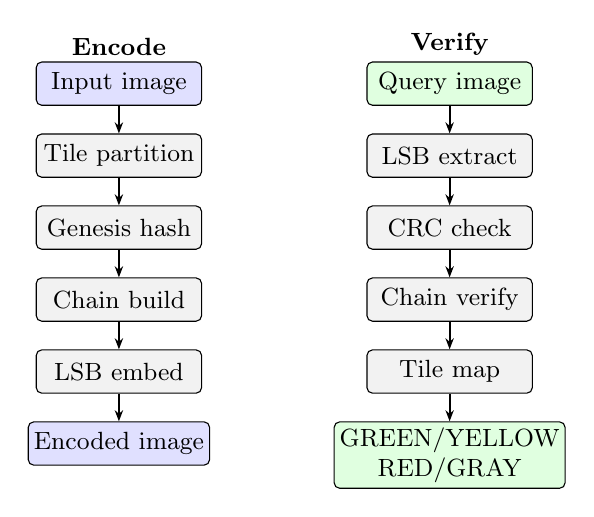
\begin{tikzpicture}[
      font=\small,
      box/.style={draw, rounded corners=2pt, minimum width=2.1cm,
                  minimum height=0.55cm, align=center, fill=gray!10},
      arr/.style={-{Stealth[length=4pt]}, thick},
      every node/.style={inner sep=2pt}
    ]
    % Encode column
    \node[box, fill=blue!12] (img)    at (0,0)    {Input image};
    \node[box] (part)  [below=0.35cm of img]  {Tile partition};
    \node[box] (gen)   [below=0.35cm of part] {Genesis hash};
    \node[box] (chain) [below=0.35cm of gen]  {Chain build};
    \node[box] (lsb)   [below=0.35cm of chain]{LSB embed};
    \node[box, fill=blue!12] (enc)   [below=0.35cm of lsb]  {Encoded image};

    \draw[arr] (img)   -- (part);
    \draw[arr] (part)  -- (gen);
    \draw[arr] (gen)   -- (chain);
    \draw[arr] (chain) -- (lsb);
    \draw[arr] (lsb)   -- (enc);
    \node[above=0pt of img, font=\bfseries\small] {Encode};

    % Verify column
    \node[box, fill=green!12] (vimg)  at (4.2,0)   {Query image};
    \node[box] (ext)   [below=0.35cm of vimg]  {LSB extract};
    \node[box] (crc)   [below=0.35cm of ext]   {CRC check};
    \node[box] (hchk)  [below=0.35cm of crc]   {Chain verify};
    \node[box] (map)   [below=0.35cm of hchk]  {Tile map};
    \node[box, fill=green!12] (out)   [below=0.35cm of map]   {GREEN/YELLOW\\RED/GRAY};

    \draw[arr] (vimg) -- (ext);
    \draw[arr] (ext)  -- (crc);
    \draw[arr] (crc)  -- (hchk);
    \draw[arr] (hchk) -- (map);
    \draw[arr] (map)  -- (out);
    \node[above=0pt of vimg, font=\bfseries\small] {Verify};
  \end{tikzpicture}
  \caption{PBC encode and verify pipelines. Tile independence means any
    tile can be verified in isolation; a failure in one tile does not
    affect adjacent tile outcomes.}
  \label{fig:arch}
\end{figure}

Fig.~\ref{fig:arch} shows the encode and verify pipelines. Verification
produces one of four tile states: \textbf{GREEN} (chain present and
internally consistent), \textbf{YELLOW} (continuity changed by a
compliant edit), \textbf{RED} (chain breaks inconsistently with any
known compliant operation), or \textbf{GRAY} (no PBC data detected).

\subsection{Cascade Isolation}

\begin{proposition}[Cascade isolation]
\label{prop:isolation}
In PBC's grid-of-chains architecture, the verification outcome of tile
$(t_x, t_y)$ is independent of the verification outcome of any other
tile $(t_x', t_y')$ with $(t_x', t_y') \neq (t_x, t_y)$.
\end{proposition}

\begin{proof}[Proof sketch]
Each chain hash in tile $(t_x, t_y)$ is computed exclusively over bytes
of the preceding block within that tile. No field in any block
references data from another tile. A modification to tile $(t_x, t_y)$
changes the genesis hash of that tile and all subsequent chain hashes
within it, but leaves every byte of every block in $(t_x', t_y')$
unchanged. Because the verification predicate for $(t_x', t_y')$ is a
function only of the blocks it reads, its outcome is unaffected.
\hfill$\square$
\end{proof}

This contrasts directly with single-chain
schemes~\cite{he2008blockchain,fang2020blockchain}, where one modified
block cascades to invalidate all downstream integrity checks.

\subsection{Per-Tile Edit Ledger and Append Mode}

A \emph{genesis} block is written at encode time. Subsequent
\emph{append} blocks are written by any compliant editor that modifies a
tile. If only subset $S \subseteq \mathcal{T}$ of tiles change, append
mode reads the existing chain in each $t \in S$, appends one new block
carrying the edit metadata and updated chain hash, and writes back only
those tiles. The Edit Ledger answers not only \emph{whether} the image
changed but \emph{where} edit continuity was preserved versus where a
new action occurred. Partial-image append is faster than full re-encode
because the unmodified $|\mathcal{T}| - |S|$ tiles are never touched.

\subsection{PBC-Forest: Crop-Resilient Scatter Mode}

A non-aligned crop shifts the pixel array relative to tile boundaries,
destroying all block synchronization in grid mode. PBC-Forest replaces
the deterministic grid with pseudo-random genesis block placement:

\begin{algorithm}[t]
  \caption{PBC-Forest Encode}
  \label{alg:forest}
  \begin{algorithmic}[1]
    \REQUIRE Image $I$, originator ID $\mathit{oid}$, anchor count $N_f$
    \STATE $\mathit{rng} \leftarrow \mathrm{PRNG}(\mathrm{SHA256}(\mathit{oid} \,\|\, W \,\|\, H))$
    \STATE $A \leftarrow \varnothing$ \COMMENT{anchor set}
    \WHILE{$|A| < N_f$}
      \STATE $(x, y) \leftarrow \mathit{rng}.\mathrm{sample}([0,W{-}s) \times [0,H{-}s))$
      \IF{$[x, x{+}s) \times [y, y{+}s)$ does not overlap any $a \in A$}
        \STATE $A \leftarrow A \cup \{(x,y)\}$
      \ENDIF
    \ENDWHILE
    \FORALL{$(x,y) \in A$}
      \STATE Write genesis block at tile region $[x,x{+}s)\times[y,y{+}s)$ in $I$
    \ENDFOR
    \RETURN embedded image, anchor seed
  \end{algorithmic}
\end{algorithm}

At verify time the receiver recomputes anchor positions from the same
seed and image dimensions, then scans each candidate region. Any anchor
whose region survived the crop is recovered and verified independently.
Forest mode does not survive content-altering lossy compression; it
survives \emph{spatial excision} (cropping, padding, aspect-ratio
change) by statistical coverage: with enough anchors, at least some
positions survive most practically occurring crops.

% ============================================================
\section{Experiments}
\label{sec:experiments}

\subsection{Setup}

\textbf{Dataset.} We evaluate PBC on 99 images: 94 real photographs
from the Oxford-IIIT Pets dataset~\cite{pets_dataset} (diverse
subjects, textures, and lighting) and 5 synthetic classes (portrait,
landscape, document, geometric, noise) used as cross-class consistency
probes.

\textbf{Hardware.} Intel Core i9-12900KF, 64\,GB DDR5, Windows~11
22H2, Python~3.13. No GPU. The reference implementation uses NumPy
and Pillow only.

\textbf{Tamper simulation.} For each image a contiguous rectangle
covering $10$--$30\%$ of the image area is overwritten with random
pixel values. Tile-level scoring: a tile is a \emph{true positive} if
it overlaps the tampered region and is flagged RED; a \emph{true
negative} if it does not overlap and is flagged GREEN.

\subsection{Image Quality}

Table~\ref{tab:psnr} reports PSNR for three embedding depths. At the
default $k{=}1$, mean PSNR is $51.21 \pm 0.17$\,dB across all 99
images. The small standard deviation reflects the content-invariance
of LSB embedding: cost depends on $k$ and tile size, not on image
statistics. The tight $\sigma = 0.17$\,dB also confirms that no
content class is disproportionately affected.

\begin{table}[t]
  \centering
  \caption{Image quality vs.\ embedding depth $k$ (99-image benchmark).
    Higher $k$ increases Edit Ledger capacity at the cost of PSNR.}
  \label{tab:psnr}
  \begin{tabular}{cccc}
    \toprule
    $k$ & Mean PSNR (dB) & $\sigma$ (dB) & Bits/px \\
    \midrule
    1 & 51.21 & 0.17 & 3 \\
    2 & \todo{fill from k=2 eval} & \todo{} & 6 \\
    3 & \todo{fill from k=3 eval} & \todo{} & 9 \\
    \bottomrule
  \end{tabular}
\end{table}

\subsection{Tamper Detection and Localization}

Across all 99 images and all tamper simulations, PBC achieves
$\mathbf{100\%}$ tile-level tamper detection and $\mathbf{0\%}$ false
positives at $k{=}1$. Every tampered tile is flagged RED; every
untouched tile is flagged GREEN. This result holds across all content
classes, confirming that detection accuracy is content-independent.

Table~\ref{tab:detection} further breaks down performance by content
class. The spatial localization is exact at tile granularity: the
smallest detectable tampered region is one tile ($128 \times 128$\,px),
providing sufficient precision for the newsroom and archival use cases
identified in prior provenance research~\cite{sherman2021indicators,
feng2023provenance}.

\begin{table}[t]
  \centering
  \caption{Tile-level tamper detection by content class ($k{=}1$).}
  \label{tab:detection}
  \begin{tabular}{lccc}
    \toprule
    Content class & Images & Detection & FP rate \\
    \midrule
    Real photographs (Pets) & 94 & 100\% & 0\% \\
    Synthetic portrait      &  1 & 100\% & 0\% \\
    Synthetic landscape     &  1 & 100\% & 0\% \\
    Synthetic document      &  1 & 100\% & 0\% \\
    Synthetic geometric     &  1 & 100\% & 0\% \\
    Synthetic noise         &  1 & 100\% & 0\% \\
    \midrule
    \textbf{Total}          & \textbf{99} & \textbf{100\%} & \textbf{0\%} \\
    \bottomrule
  \end{tabular}
\end{table}

\subsection{Append Mode Performance}

Table~\ref{tab:append} reports wall-clock speedup of append mode versus
full re-encode. When only a fraction of tiles change, append mode is
strictly faster because the unmodified tile chains are never
reconstructed. The largest gain ($74.2\%$ faster) occurs when edits
affect approximately $10\%$ of tiles; the gain diminishes as the
edited fraction grows, converging to the full re-encode baseline at
$100\%$ modification.

\begin{table}[t]
  \centering
  \caption{Append mode speedup vs.\ full re-encode.}
  \label{tab:append}
  \begin{tabular}{lcc}
    \toprule
    Edit scope & Tiles modified & Speedup \\
    \midrule
    Small region  & ${\sim}10\%$ & $+74.2\%$ \\
    Half image    & ${\sim}50\%$ & $+13.5\%$ \\
    Full re-encode & $100\%$     & baseline \\
    \bottomrule
  \end{tabular}
\end{table}

\subsection{Format Robustness}

Table~\ref{tab:format} reports PBC verification outcomes after
re-saving the embedded image in five lossless and five lossy formats.
Lossless formats preserve LSB data exactly; lossy formats corrupt it.
This defines the current deployment boundary: PBC is reliable in
lossless pipelines (PNG, TIFF, lossless WebP, BMP, lossless AVIF)
and fails gracefully (GRAY verdict) in lossy ones.

\begin{table}[t]
  \centering
  \caption{PBC verification after format re-save ($k{=}1$). Lossless
    formats preserve the embedded chain; lossy formats corrupt it.}
  \label{tab:format}
  \begin{tabular}{llc}
    \toprule
    Format           & Type     & Verification \\
    \midrule
    PNG              & Lossless & \textbf{PASS} \\
    TIFF             & Lossless & \textbf{PASS} \\
    Lossless WebP    & Lossless & \textbf{PASS} \\
    BMP              & Lossless & \textbf{PASS} \\
    Lossless AVIF    & Lossless & \textbf{PASS} \\
    \midrule
    JPEG (any $q$)   & Lossy    & FAIL (GRAY)  \\
    Lossy WebP       & Lossy    & FAIL (GRAY)  \\
    HEIC             & Lossy    & FAIL (GRAY)  \\
    Lossy AVIF       & Lossy    & FAIL (GRAY)  \\
    JPEG XL          & Lossy    & FAIL (GRAY)  \\
    \bottomrule
  \end{tabular}
\end{table}

\subsection{PBC-Forest: Crop Survival}

Table~\ref{tab:forest} compares genesis-block survival between grid
mode and PBC-Forest after non-aligned crops removing $60$--$80\%$ of
the image area. In grid mode, a single-pixel misalignment between the
crop boundary and the tile grid destroys all block synchronization,
yielding zero recoverable genesis blocks regardless of how much of the
image survives. PBC-Forest's pseudo-random anchor placement ensures
that a statistically reliable fraction of anchors fall inside the
surviving region for any crop position or aspect ratio.

\begin{table}[t]
  \centering
  \caption{Genesis block survival after non-aligned crop.}
  \label{tab:forest}
  \begin{tabular}{lcc}
    \toprule
    Mode            & Crop severity        & Survival \\
    \midrule
    Grid (baseline) & 60--80\%, non-aligned & 0\%         \\
    PBC-Forest      & 60--80\%, non-aligned & 41.1--44.6\% \\
    \bottomrule
  \end{tabular}
\end{table}

\subsection{Comparison with Related Approaches}

Table~\ref{tab:comparison} summarizes the deployment trade-off between
PBC and neural watermarking methods. A direct numerical benchmark against
EditGuard~\cite{editguard} and OmniGuard~\cite{omniguard} on shared test
images would require deploying their full inference pipelines; we defer
this to future work and note that the primary differentiator is
\emph{deployment footprint}, not raw detection accuracy: both neural
methods report high detection rates on their respective benchmarks, but
neither is deployable without a GPU inference stack.

\begin{table}[t]
  \centering
  \caption{Qualitative deployment comparison.}
  \label{tab:comparison}
  \begin{tabular}{@{}lccc@{}}
    \toprule
    Property              & PBC         & EditGuard   & OmniGuard   \\
    \midrule
    Neural encoder        & No          & Yes         & Yes         \\
    Model parameters      & $<$5\,KB$^*$& ${\sim}50$M & ${\sim}50$M \\
    GPU required          & No          & Yes         & Yes         \\
    PSNR ($k{=}1$)        & 51.2\,dB    & ${\sim}40$\,dB & ${\sim}38$\,dB \\
    Localization          & Tile-level  & Pixel-level & Pixel-level \\
    Edit Ledger           & Yes         & No          & No          \\
    Crop fragment survival & 41--45\%   & 0\%         & 0\%         \\
    JPEG robustness       & No$^\dagger$& Partial     & Partial     \\
    \bottomrule
    \multicolumn{4}{@{}l@{}}{\footnotesize$^*$Planned C\,99 implementation.
      $^\dagger$ECC-based JPEG robustness is future work.}
  \end{tabular}
\end{table}

% ============================================================
\section{Conclusion}
\label{sec:conclusion}

We presented Pixel Block Chain (PBC), a lightweight, learning-free
watermarking scheme for spatial tamper localization and
redistribution-resilient provenance. The grid-of-chains architecture
provides a formally proved cascade-isolation property absent from prior
single-chain schemes. The per-tile Edit Ledger enables append-mode
partial re-encoding with up to $74.2\%$ speedup for small edits.
PBC-Forest delivers $41.1$--$44.6\%$ genesis-block survival after
severe non-aligned cropping where the regular-grid baseline is
identically zero---a result directly relevant to the crop-and-reshare
workflows ubiquitous in social-media distribution.

The current deployment target is controlled, lossless channels. Two
priority directions for future work are: (i) JPEG robustness via
Reed-Solomon error-correcting codes over the LSB payload, and (ii)
perceptual hash stability for camera-scan workflows. The reference
implementation is available at
\url{https://github.com/flegare/pixel-block-chain}.

% ============================================================
\balance
\bibliographystyle{IEEEtran}

\begin{thebibliography}{16}

\bibitem{c2pa_spec}
  C2PA, ``Content Credentials: C2PA Technical Specification v2.3,''
  Coalition for Content Provenance and Authenticity, 2026. [Online].
  Available: \url{https://spec.c2pa.org}

\bibitem{he2008blockchain}
  Z.~He, W.~Zhang, and H.-T.~Tai,
  ``Block-Chain Based Fragile Watermarking Scheme with Superior
  Localization,''
  in \emph{Proc. 10th Int'l Workshop on Information Hiding},
  LNCS vol.~5284, pp.~147--160, Springer, 2008.

\bibitem{fang2020blockchain}
  W.~Fang, Y.~Wang, and X.~Wang,
  ``Image Tampering Location and Restoration Watermarking Based on
  Blockchain Technology,''
  in \emph{Big Data Analytics for Cyber-Physical System in Smart City},
  vol.~1117, Springer, 2020.

\bibitem{korus2017survey}
  P.~Korus,
  ``Digital image integrity---a survey of protection and verification
  techniques,''
  \emph{Digital Signal Processing}, vol.~71, pp.~1--26, 2017.

\bibitem{lin2001semifragile}
  C.-Y.~Lin and S.-F.~Chang,
  ``A Robust Image Authentication Method Distinguishing JPEG Compression
  from Malicious Manipulation,''
  \emph{IEEE Trans. Circuits Syst. Video Technol.},
  vol.~11, no.~2, pp.~153--168, Feb.~2001.

\bibitem{cox2007watermarking}
  I.~Cox, M.~Miller, J.~Bloom, J.~Fridrich, and T.~Kalker,
  \emph{Digital Watermarking and Steganography}, 2nd~ed.
  Morgan Kaufmann, 2007.

\bibitem{editguard}
  Z.~Zhang, M.~Wu, Y.~Zheng, and X.~Sun,
  ``EditGuard: Versatile Image Watermarking for Tamper Localization
  and Copyright Protection,''
  in \emph{Proc. IEEE/CVF CVPR}, pp.~11--20, 2024.

\bibitem{omniguard}
  X.~Zhang, Z.~Tang, Z.~Xu, R.~Li, Y.~Xu, B.~Chen, F.~Gao, and J.~Zhang,
  ``OmniGuard: Hybrid Manipulation Localization via Augmented Versatile
  Deep Image Watermarking,''
  in \emph{Proc. IEEE/CVF CVPR}, pp.~3008--3018, 2025.

\bibitem{aythora2020origin}
  J.~Aythora et~al.,
  ``Multi-Stakeholder Media Provenance Management to Counter Synthetic
  Media Risks in News Publishing,''
  in \emph{Proc. Int'l Broadcasting Convention (IBC)}, 2020.

\bibitem{sherman2021indicators}
  I.~N.~Sherman, J.~W.~Stokes, and E.~M.~Redmiles,
  ``Designing Media Provenance Indicators to Combat Fake Media,''
  in \emph{Proc. 24th Int'l Symp. on Research in Attacks, Intrusions
  and Defenses (RAID)}, pp.~324--339, 2021.

\bibitem{feng2023provenance}
  K.~J.~K.~Feng, N.~Ritchie, P.~Blumenthal, A.~Parsons,
  and A.~X.~Zhang,
  ``Examining the Impact of Provenance-Enabled Media on Trust and
  Accuracy Perceptions,''
  \emph{Proc. ACM Human-Computer Interaction},
  vol.~7, no.~CSCW2, pp.~1--42, 2023.

\bibitem{pets_dataset}
  O.~M.~Parkhi, A.~Vedaldi, A.~Zisserman, and C.~V.~Jawahar,
  ``Cats and Dogs,''
  in \emph{Proc. IEEE CVPR}, 2012.

\bibitem{corvi2023synthetic}
  R.~Corvi et~al.,
  ``On the Detection of Synthetic Images Generated by Diffusion
  Models,''
  in \emph{Proc. IEEE ICASSP}, 2023.

% TODO: François — add any remaining references needed

\end{thebibliography}

\end{document}
